\documentclass[../main.tex]{subfiles}

\usepackage{graphicx}
\graphicspath{ {../resources/} }

\setcounter{section}{5}

\begin{document}

\begin{exercise}
  Let $T \in \LT(V)$. Show that $9$ is an eigenvalue of $T^2$ $\iff$ $3$ or $-3$ is an eigenvalue of $T$.
\end{exercise}
\begin{proof}
  ~
  \begin{itemize}
    \item $(\Rightarrow)$ We have $T^2 - 9I$ is not injective since $9$ is an eigenvalue of $T^2$,
          then $(T - 3I)(T + 3I) = T^2 - 9I$ is not injective means one of $T - 3I$ and $T + 3I$
          is not injective, thus $3$ or $-3$ is an eigenvalue of $T$.
    \item $(\Leftarrow)$ Similarly, we have $(T - 3I)(T + 3I)v = (T^2 - 9I)v = 0$ (if $3$ is an eigenvalue of $T$)
          or $(T + 3I)(T - 3I)v = (T^2 - 9I)v = 0$ (if $-3$ is an eigenvalue of $T$).
  \end{itemize}
\end{proof}

\begin{exercise}
  Let $V$ a vector space over $\mathbb{C}$ and $T \in \LT(V)$ has no eigenvalue.
  Show that any subspace of $V$ that is invariant under $T$ is either $\0$
  or infinite dimension.
\end{exercise}
\begin{proof}
  Let $U \subseteq V$ a subspace that is invariant under $T$, and non-zero $u \in U$.
  We can repeatly apply $T$ to $u$, say $u, Tu, T^2u, \cdots$. Suppose $k > 0$ is minimum such that
  $u, Tu, \cdots, T^ku$ is linear dependent, we have $p \in \mathcal{P}(\mathbb{C})$ with $\deg p = k$ such that $p(T) = 0$.
  Clearly $p$ is not constants, thus it has a zero since $p$ is a polynomial of complex coefficient.
  Thus such zero is an eigenvalue of $T$.
\end{proof}

\begin{exercise}
  Let $n > 1$ an integer, and $T \in \LT(F^n)$ is defined by:
  \[
  T(\join{x}{n - 1}) = (\join[+]{x}{n - 1}, \cdots, \join[+]{x}{n - 1})
  \]
  \begin{itemize}
    \item Find all eigenvalue and eigenvector of $T$.
    \item Find the minimal polynomial of $T$.
  \end{itemize}
\end{exercise}
\begin{proof}
  ~
  \begin{itemize}
    \item Observe that $\rangev T = \spanv((1, \cdots, 1))$, thus $T(1, \cdots, 1) = n(1, \cdots, 1)$.
    \item Observe that $T(\join{x}{n - 1}) = (\join[+]{x}{n - 1})(1, \cdots, 1)$ and \\
          $T^2(\join{x}{n - 1}) = n(\join[+]{x}{n - 1})(1, \cdots, 1)$,
          thus $p(T) = nT - T^2 = 0$.
  \end{itemize}
\end{proof}

Exercise 4 is kinda hard, sorry.

\setcounter{exercise}{5}
\begin{exercise}
  Let $T \in \LT(F^2)$ is defined by $T(w, z) = (-z, w)$.
  Find the minimal polynomial of $T$.
\end{exercise}
\begin{proof}
  Observe that $T^2(w, z) = T(-z, w) = (-w, -z) = (-1) (w, z)$,
  thus the minimal polynomial of $T$ is $p(T) = I + T^2$.
\end{proof}

\begin{exercise}
  \begin{itemize}
    \item Given an example that the minimal polynomial of $ST$ is not equal to $TS$'s.
    \item Suppose $V$ is finite and $S, T \in \LT(V)$. Show that the minimal polynomial of $ST$
          is equal to $TS$'s if one of $S$ and $T$ is invertible.

          Hint: Show that $S$ is invertible and $p \in \mathcal{P}(F)$ implies $p(TS) = \inv{S} p(ST) S$.
  \end{itemize}
\end{exercise}
\begin{proof}
  ~
  \begin{itemize}
    \item The idea is to find $S, T$ such that $ST \neq 0$ but $TS = 0$. 
          We can find $S(x, y) = (x, 0)$ and $T(x, y) = (y, 0)$ holds:
          \begin{align*}
            (ST)(x, y) = S(y, 0) = (y, 0) \\
            (TS)(x, y) = T(x, 0) = (0, 0)
          \end{align*}
          Thus the minimal polynomial of $ST$ is not $0$ but $TS$ one does.
    \item Suppose $S$ is invertible and $p \in \LT(F)$ is the minimal polynomial of $TS$,
          then $p(TS) = \inv{S} p(ST) S$ since $i$-th term of $\inv{S} p(ST) S$
          has form $\inv{S} c_i (ST)^i S = c_i (\inv{S} S)(TS)^{i - 1}(TS) = c_i (TS)^i$.
          Thus $\inv{S} p(ST) S = 0$ and then $p(ST) = 0$.
          We will show that $p$ is the minimal polynomial of $ST$, suppose $q \in \LT(F)$
          such that $q(ST) = 0$, then $0 = \inv{S} q(ST) S = q(TS)$, therefore $\deg q = \deg p$.
          Hence $p$ is the minimal polynomial of $ST$.
  \end{itemize}
\end{proof}

\begin{exercise}
  Let $T \in \LT(R^2)$ is the opeartor that "rotates 1 degree counterclockwise",
  find the minimal polynomial of $T$.

  Note that it is \textbf{NOT} $x^{180} + 1$ even $T^{180} = -I$.
\end{exercise}
\begin{proof}
  Note that there is some $\lambda$ such that $Tv - \lambda v = \alpha T^2 v$ (We can show that $\lambda = \alpha$),
  however the calculation is too complicate.

  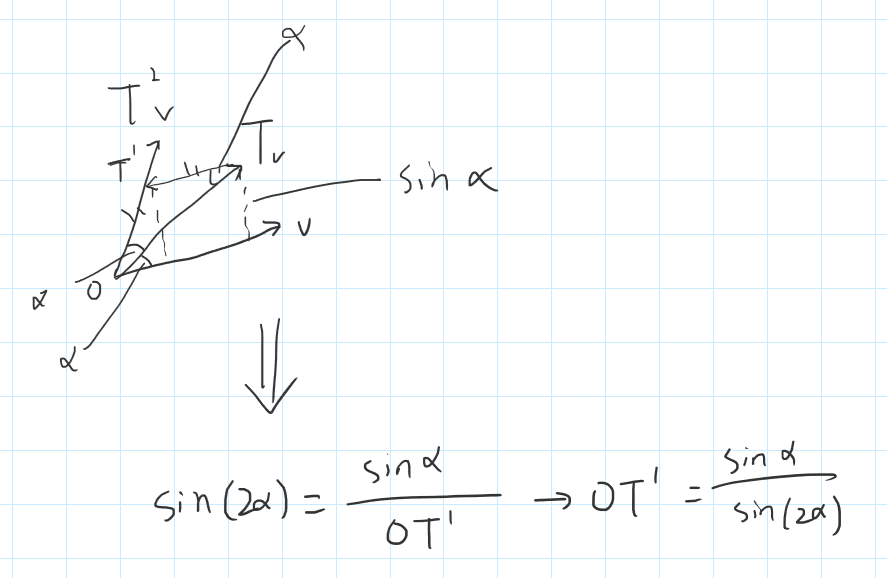
\includegraphics[scale=0.6]{E5B-8-resource}

  $\lambda$ should be $\frac{\sin(1^{\circ})}{\sin(2^\circ)}$, thus
  $p(T) = - \lambda I + T - \lambda T^2$.

  We suppose all $v$ below has length $1$, thus $v = (\cos \theta, \sin \theta)$,
  this doesn't lose the generalizability since $p(T)(\alpha v) = \alpha (p(T)v)$.

  For the first component of $p(T)v = - \lambda v + Tv - \lambda T^2v$, we have:
  \begin{align*}
     & \frac{\sin(1^\circ)}{\sin(2^\circ)} (- \cos \theta - \cos (\theta + 2^\circ)) \\
    =& \frac{\sin(1^\circ)}{\sin(2^\circ)} (- \cos \theta - (\cos \theta \cos(2^\circ) - \sin \theta \sin (2^\circ))) \\
    =& \frac{\sin(1^\circ)}{\sin(2^\circ)} (- \cos \theta - \cos \theta \cos(2^\circ)) + \sin \theta \sin (1^\circ) \\
    =& \cos \theta \frac{\sin(1^\circ)}{\sin(2^\circ)} (- 1 - \cos(2^\circ)) + \sin \theta \sin (1^\circ) \\
  \end{align*}
  where $\sin \theta \sin(1^\circ)$ cancels a part of
  $(Tv)_1 = \cos(\theta + 1^\circ) = \cos \theta \cos (1^\circ) - \sin \theta \sin (1^\circ)$.
  Thus we will show that $\frac{\sin(1^\circ)}{\sin(2^\circ)} (- 1 - \cos(2^\circ)) = - \cos (1^\circ)$.
  \begin{align*}
     & \frac{\sin(1^\circ)}{\sin(2^\circ)} (- 1 - \cos(2^\circ)) \\
    =& \frac{\sin(1^\circ)}{2\sin(1^\circ)\cos(1^\circ)} (- (\cos^2(1^\circ) + \sin^2(1^\circ)) - \cos^2(1^\circ) + \sin^2(1^\circ)) \\
    =& \frac{1}{2\cos(1^\circ)} (- \cos^2(1^\circ) - \cos^2(1^\circ)) \\
    =& \frac{1}{2\cos(1^\circ)} (- 2 \cos^2(1^\circ)) \\
    =& - \cos(1^\circ) \\
  \end{align*}

  For the second component of $p(T)v$, we have:
  \begin{align*}
     & \frac{\sin(1^\circ)}{\sin(2^\circ)} (- \sin \theta - \sin (\theta + 2^\circ)) \\
    =& \frac{\sin(1^\circ)}{\sin(2^\circ)} (- \sin \theta - \sin \theta \cos(2^\circ) - \cos \theta \sin (2^\circ)) \\
    =& \sin \theta \frac{\sin(1^\circ)}{\sin(2^\circ)} (- 1 - \cos(2^\circ)) - \cos \theta \sin (1^\circ) \\
  \end{align*}
  similarly, we have $p(T)v_2 = \sin (\theta + 1^\circ) = \sin \theta \cos (1^\circ) + \cos \theta \sin (1^\circ)$ we will show that $\frac{\sin(1^\circ)}{\sin(2^\circ)} (- 1 - \cos(2^\circ)) = - \cos (1^\circ)$,
  which is proven above.
\end{proof}

\begin{exercise}
  Let $T \in \LT(V)$ such that for some basis of $V$, $\mathcal{M}(T)$ consists of
  rational numbers. Try to explain why the coefficients of the minimal polynomial of $T$
  is rational numbers.
\end{exercise}
\begin{proof}
  I don't know, because $\mathbb{Q}$ is also a field?
\end{proof}

\setcounter{exercise}{10}
\begin{exercise}
  Let $V$ a vector space and $\dim V = 2$ and $T \in \LT(V)$ such that $\mathcal{M}(T)$
  for some basis of $V$ is $\begin{bmatrix}
    a & c \\
    b & d \\
  \end{bmatrix}$.
  Show that:
  \begin{itemize}
    \item $T^2 - (a + d)T + (ad - bc)I = 0$
    \item the minimal polynomial of $T$ is:
          \[
          \begin{cases}
            z - a \quad & \text{if } b = c = 0 \text{ and } a = d \\
            z^2 - (a + d) z + (ad - bc) \quad & \text{otherwise}
          \end{cases}
          \]
  \end{itemize}
\end{exercise}
\begin{proof}
  \def\MT{\begin{bmatrix} a & c \\ b & d \end{bmatrix}}
  ~
  \begin{itemize}
    \item \begin{align*}
             & \mathcal{M}(T^2 - (a + d) T + (ad - bc)I) \\
            =& \MT^2 - (a + d)\MT + (ad - bc)I \\
            =& \begin{bmatrix} 
              a^2 + bc & ac + bd \\
              ab + bd & bc + d^2 \\
            \end{bmatrix} - \begin{bmatrix}
              a^2 + ad & ac + cd \\
              ab + bd & ad + d^2 \\
            \end{bmatrix}
            + \begin{bmatrix}
              ad - bc & 0 \\
              0 & ad - bc \\
            \end{bmatrix}
          \end{align*}
    \item If $b = c = 0$ and $a = d$, then $T$ is a scalar multiple of identity operator,
          thus $T = aI$ and $p(T) = -aI + T = 0$.
          Otherwise, $T^2 - (a + d)T + (ad - bc)I = 0$.
  \end{itemize}
\end{proof}

\setcounter{exercise}{12}
\begin{exercise}
  Let $V$ finite, $T \in \LT(V)$, $p \in \mathcal{P}(F)$.
  Show that there is a unique $r \in \mathcal{P}(F)$ such that $p(T) = r(T)$
  where $\deg p$ is less than the degree of the minimal polynomial of $T$.
\end{exercise}
\begin{proof}
  Let $q$ the minimal polynomial of $T$.

  If $\deg p < \deg q$, then $r = p$. The uniqueness is guaranteed by
  $\deg p < \deg q$ (try $(p - s)(T)$ where $p(T) = s(T)$ and $\deg s < \deg q$).

  If $\deg p >= \deg q$, then $p = sq + r$ where $s, r \in \mathcal{P}(F)$
  with $\deg r < \deg q$.Then $p(T) = s(T)q(T) + r(T) = r(T)$ since $q(T) = 0$.
  The uniqueness is guaranteed by the property of division.
\end{proof}

\begin{exercise}
  Let $V$ finite, $T \in \LT(V)$ with minimal polynomial $p(z) = 4 + 5z - 6z^2 - 7z^3 + 2z^4 + z^5$.
  Find the minimal polynomial of $\inv{T}$.
\end{exercise}
\begin{proof}
  Suppose $p$ is the minimal polynomial of $T$, then we can
  repeatly apply $\inv{T}$ to $p(T)$, say $T^{-(\deg p)}(p(T))$,
  then it should be $0$, and the coefficients are reversed,
  that is, $p_{\deg p}I + p_{\deg p - 1}\inv{T} + \cdots + p_0(\inv{T})^{\deg p}$.

  So the answer is $1 + 2z^1 - 7z^2 - 6z^3 + 5z^4 + 4z^5$.
\end{proof}

\setcounter{exercise}{15}
\begin{exercise}
  Let $\join{a}{n - 1} \in F$ and $T$ an operator over $F^n$.
  Its matrix (about the standard basis) is:
  \[
  \begin{bmatrix}
    0 &   &        &   &   & - a_0 \\
    1 & 0 &        &   &   & - a_1 \\
      & 1 & \ddots &   &   & - a_2 \\
      &   & \ddots &   &   & \vdots \\
      &   &        & 1 & 0 & - a_{n - 2} \\
      &   &        &   & 1 & - a_{n - 1} \\
  \end{bmatrix}
  \].
  Show that the minimal polynomial of $T$ is:
  \[
  p(z) = a_0 + a_1 z + \cdots + a_{n - 1}z^{n - 1} + z^n
  \]
\end{exercise}
\begin{proof}
  We first need some property of this matrix, we will see it moves
  all number to the left when we repeatly self-multily $T$.
  We can see the $k$-th column of $T^p$
  is equal to $k + 1$-th column of $T^{p - 1}$, thus
  it is also equal to $i$-th column if $T^j$
  where $1 \le i, j \le n$ and $i + j = k + p$.
  In fact, $j$ can be $0$ and we have $T^0 = I$ and the property
  still holds.

  Then, the $i$-th column of $T^n$ is equal to $n$-th column (the last one) of $T^i$,
  and it is produced by $T^{i - 1}\begin{bmatrix}
    - a_0 \\
    - a_1 \\
    \vdots \\
    - a_{n - 1}
  \end{bmatrix}$, which is equal to
  \[
  T^n_i = - a_0 T^{i - 1}_1 - a_1 T^{i - 1}_2 - \cdots - a_{n - 1} T^{i - 1}_n
  \]
  which is equal to $T^n v_i$ where $v_i$ is $i$-th standard basis of $F^n$,
  that is, $\begin{bmatrix}
    0 \\
    \vdots \\
    1 \\
    \vdots \\
    0
  \end{bmatrix}$. We may rewrite the equation into
  \[
  T^nv = -a_0 T^0v - a_1T^1v - \cdots - a_{n - 1}T^{n - 1}v
  \]
  where $T^0v = T^0_i = T^{i - 1}_1$, $T^1v = T^1_i = T^{i - 1}_2$ and so on.

  Thus all $v$ vector in standard basis has $p(T)v = 0$, thus $p(T) = 0$.

  For minimal, we can see $T$ is invertible, thus $p(T)v_1 = 0$
  (recall that $T$ moves number to the left, thus the first column of $T^i$ is the $i$-th columns of $T$).
  means there is a (non-zero) linear combination of columns of $T$ that is equal to $0$.
  Thus $\deg p \ge n$ since $T$ the columns are linear independent.
\end{proof}

\begin{exercise}
  Let $V$ finite and $T \in \LT(V)$ and $p$ is the minimal polynomial of $T$.
  Let $\lambda \in F$, show that the minimal polynomial of $T - \lambda I$
  is $q(z) = p(z + \lambda)$.
\end{exercise}
\begin{proof}
  $q(T - \lambda I) = p((T - \lambda I) + \lambda I) = p(T) = 0$.
  Suppose $r$ is the minimal polynomial of $T - \lambda I$,
  then $s(z) = r(z - \lambda)$ and $s(T) = r(T - \lambda I) = 0$, thus $\deg r = \deg p = \deg q$.
\end{proof}

\begin{exercise}
  Let $V$ finite and $T \in \LT(V)$, and $p$ is the minimal polynomial of $T$.
  Let $\lambda \in F$ that $\lambda \neq 0$, show that
  the minimal polynomial of $\lambda T$ is $q(z) = \lambda^{\deg p} p(\frac{z}{\lambda})$.
\end{exercise}
\begin{proof}
  $q(\lambda T) = \lambda^{\deg p}p(\frac{1}{\lambda}(\lambda T)) = \lambda^{\deg p} p(T) = 0$.
  $\lambda^{\deg p}$ only makes $q$ a monic polynomial.

  Suppose $r$ is the minimal polynomial of $\lambda T$, then $s(z) = \frac{1}{\lambda^{\deg p}}r(\lambda z)$
  and $s(T) = \frac{1}{\lambda^{\deg p}}r(\lambda T) = 0$, thus $\deg s = \deg r = \deg p = \deg q$.
\end{proof}

\begin{exercise}
  Let $V$ finite and $T \in \LT(V)$. Let $\mathcal{E} \subseteq \LT(V)$ a subspace,
  defined by
  \[
  \mathcal{E} = \set{q(T)}{q \in \mathcal{P}(F)}
  \].

  Show that $\dim \mathcal{E}$ is equal to the degree of the minimal polynomial of $T$.
\end{exercise}
\begin{proof}
  We can see $I, T, T^2, \cdots, T^{\deg p - 1}$ is linear independent (since $p$ is the minimal polynomial of $T$) where $p$ is
  the minimal polynomial of $T$. For any $q \in \mathcal{P}(F)$
  where $\deg q \ge \deg p$, then $q = sp + r$ where $s, r \in \mathcal{P}(F)$
  and $\deg r < \deg p$, therefore $q(T) = s(T)p(T) + r(T) = r(T) \in \spanv(I, T, T^2, \cdots, T^{\deg p - 1})$.
\end{proof}

\begin{exercise}
  let $T \in \LT(F^4)$, which eigenvalues are $3, 5, 8$. Show that $(T - 3I)^2(T - 5I)^2(T - 8I)^2 = 0$.
\end{exercise}
\begin{proof}
  Suppose $p$ is the minimal polynomial of $T$, then $p(z) = c(z - 3)(z - 5)(z - 8)q(z)$
  since $3, 5, 8$ are the eigenvalue of $T$, thus the zeros of $p$.
  Note that $\deg q \le 1$ since $\deg p \le \dim F^4 = 4$.
  Since there is no other eigenvalue (thus zero) than $3, 5, 8$, $q$ is either $1$
  or one of $z - 3$, $z - 5$, $z - 8$, thus $(z - 3)^2(z - 5)^2(z - 8)^2$ is 
  polynomial multiple of $p$, therefore $(T - 3I)^2(T - 5I)^2(T - 8I)^2 = 0$.
\end{proof}

\begin{exercise}
  Let $V$ finite and $T \in \LT(V)$. Show that the degree of the minimal polynomial of $T$
  caps at $1 + \dim \rangev T$.
\end{exercise}
\begin{proof}
  IDk
\end{proof}

\begin{exercise}
  Let $V$ finite and $T \in \LT(V)$.
  Show that $T$ is invertible $\iff$ $I \in \spanv(T, T^2, \cdots, T^{\dim V})$.
\end{exercise}
\begin{proof}
  ~
  \begin{itemize}
    \item $(\Rightarrow)$ Suppose $T$ is invertible, then the minimal polynomial $p$
          of $T$ satisfies $p(0) \neq 0$ (since $p(0) = 0$ implies $0$ is a eigenvalues of $T$).
          We know $\deg p \le \dim V$, thus there is a linear combination of $T, T^2, \cdots, T^{\dim V}$
          that is equal to a scalar multiple of $I$, therefore $I \in \spanv(T, T^2, \cdots, T^{\dim V})$.
    \item $(\Leftarrow)$ Suppose $I = \lambda_1 T + \lambda_2 T^2 + \cdots + \lambda_{\dim V} T^{\dim V}$,
          then $I = T(\lambda_1 I + \lambda_2 T + \cdots + \lambda_{\dim V}T^{\dim V - 1}) = (\lambda_1 I + \lambda_2 T + \cdots + \lambda_{\dim V}T^{\dim V - 1})T$,
          thus $T$ is invertible.
  \end{itemize}
\end{proof}


\begin{exercise*}
  Let $V$ a vector space and $T \in \LT(V)$, $v, Tv, \cdots, T^kv$ a list of linear independent
  vectors but $v, Tv, \cdots, T^{k + 1}v$ isn't. Show that $T^{k + i}v \in \spanv(v, Tv, \cdots, T^kv)$ for all $0 < i$.
\end{exercise*}
\begin{proof}
  Induction on $i$.
  \begin{itemize}
    \item Base$(i = 1)$: By assumption.
    \item Ind$(i = i + 1)$: $T^{k + i + 1}v = T(T^{k + i}v)$, since $T^{k + i}v \in \spanv(v, Tv, \cdots, T^k v)$,
          thus it can be write as a linear combination of $v, Tv, \cdots, T^kv$,
          say $T(\lambda_0 v + \lambda_1 Tv + \cdots + \lambda_k T^kv)$,
          then $\lambda_0 Tv + \lambda_1 T^2v + \cdots, + \lambda_k T^{k + 1} v \in \spanv(v, Tv, \cdots, T^kv)$
          since $T^{k + 1} v \in \spanv(v, Tv, \cdots, T^k v)$.
  \end{itemize}
\end{proof}

\begin{exercise}
  Let $V$ finite and $T \in \LT(V)$. Let $n = \dim V$, show that for any $v \in V$,
  $\spanv(v, Tv, \cdots, T^{n - 1}v)$ is invariant under $T$.
\end{exercise}
\begin{proof}
  Note that the list $v, Tv, \cdots, T^{n - 1}v$ has length $n = \dim V$, thus
  for the list $v, Tv, \cdots, T^nv$ is linear dependent, thus $T^nv$ must
  be a linear combination of $v, Tv, \cdots, ^{n - 1}v$.
  \begin{itemize}
    \item If $v, Tv, \cdots, T^{n - 1}v$ is linear dependent, then $T^nv \in \spanv(v, Tv, \cdots, T^{n - 1}v)$
          (by our lemma exercise).
    \item Otherwise, the list $v, Tv, \cdots, T^n v$ is linear dependent while $v, Tv, \cdots, T^{n - 1}v$ isn't,
          therefore $T^nv$ is a linear combination of $v, Tv, \cdots, T^{n - 1}v$.
  \end{itemize}
\end{proof}

\setcounter{theorem}{28}
\begin{theorem}
  $q(T) = 0 \iff$ $q$ is a polynomial multiple of the minimal polynomial of $T$.
\end{theorem}
\begin{proof}
  \begin{itemize}
    \item $(\Rightarrow)$ Let $p$ the minimal polynomial of $T$, consider
          $q = sp + r$ where $\deg r < \deg p$, we may suppose $r \neq 0$.
          Then $0 = q(T) = s(T)p(T) + r(T) = r(T)$, which contradict
          to the assumption that $p$ is the minimal polynomial of $T$.
    \item $(\Leftarrow)$ Trivial.
  \end{itemize}
\end{proof}

\setcounter{exercise}{24}
\begin{exercise}
  Let $V$ finite, $T \in \LT(V)$, subspace $U \subseteq V$ is invariant under $T$.
  \begin{itemize}
    \item Show that the minimal polynomial of $T$ is polynomial multiple of
          the minimal polynomial of $T/U$.
    \item Show that
          \[
          (\text{the minimal polynomial of } T\big|_U) \times (\text{the minimal polynomial of } T/U)
          \]
          is a polynomial multiple of the minimal polynomial of $T$.
  \end{itemize}
\end{exercise}
\begin{proof}
  \begin{itemize}
    \item Let $p$ the minimal polynomial of $T$, then $p(T/U)(v + U) = p(T)v + U = 0 + U$ for
          any $v + U \in V/U$, thus $p(T/U) = 0$, therefore $p$ is a polynomial multiple of
          the minimal polynomial of $T/U$.
    \item Let $p$ the minimal polynomial of $T\big|_U$ and $q$ the minimal polynomial of $T/U$.
          Then $(pq)(T)v = (p(T)q(T))v = p(T)(q(T)v)$ where $q(T)v \in U$,
          thus $p(T)(q(T)v) = 0$.
  \end{itemize}
\end{proof}

\begin{exercise}
  Let $V$ finite, $T \in \LT(V)$, $U$ is invariant under $T$.
  Show that the set of eigenvalues of $T$ is equal to the
  union of eigenvalues of $T\big|_U$ and $T/U$.
\end{exercise}
\begin{proof}
  This theorem separate the eigenvalues into two parts: eigenvectors
  in $U$ and eigenvectors not in $U$ (may have intersection).
  \begin{itemize}
    \item $(\subseteq)$ For any $Tv = \lambda v$ where non-zero $v \in V$.
          If $v \in U$, then $T\big|_U(v) = Tv = \lambda v$.
          If $v \notin U$, then $(T/U)(v + U) = Tv + U = \lambda v + U = \lambda (v + U)$.
    \item $(\supseteq)$ For any $T\big|_U(v) = \lambda v$, we have $T\big|_U(v) = Tv = \lambda v$.
          The case of $T/U$ is proven in Exercise 5.38 of E5A.
  \end{itemize}
\end{proof}

We will use this conclusion several times, so we prove it first.
\begin{exercise*}
  Let $p, q$ two non-constant \textbf{monic} polynomial and $p = sq$, $q = tp$
  where $s, t$ two non-zero polynomial. Show that $p = q$.
\end{exercise*}
\begin{proof}
  We have $p = stp$, thus $st = 1$ and $\deg s = \deg t = 0$.
  Furthermore, we have $p = sq$ where $p$ and $q$ are monic,
  thus $s$ must be $1$, similar to $t$, hence $s = t = 1$ and $p = q$.
\end{proof}

\begin{exercise}
  Let $F = R$ and $V$ finite and $T \in \LT(V)$.
  Show that the minimal polynomial of $T_C$ is equal to the $T$ one.
\end{exercise}
\begin{proof}
  Let $p$ the minimal polynomial of $T$ and $q$ the minimal polynomial of $T_C$.
  We have:
  \begin{align*}
     & p(T_C)(v + iu) \\
    =& p(T)v + ip(T)u \\
    =& 0v + i0u \\
    =& 0
  \end{align*}
  and
  \begin{align*}
     & q(T)(v) \\
    =& q(T_C)(v + i0) \\
    =& 0
  \end{align*}
  thus $p = sq$ and $q = tp$ where $s, t$ are non-zero polynomials,
  therefore $p = q$.
\end{proof}

\begin{exercise}
  Let $V$ finite and $T \in \LT(V)$. Show that
  the minimal polynomial of $T^\prime \in \LT(V^\prime)$
  is equal to the $T$ one.
\end{exercise}
\begin{proof}
  Let $p$ the minimal polynomial of $T$ and $p^\prime$ the minimal polynomial of $T^\prime$.

  For any $\varphi \in V^\prime$ and $v \in V$, we have
  $p(T^\prime)(\varphi)(v) = \varphi (p(T)v) = \varphi0 = 0$ (since $\varphi$ is linear),
  thus $p(T^\prime)(\varphi) = 0$, therefore $p(T^\prime) = 0$.

  For any $v \in V$, $p^\prime(T)v = \varphi_1(p^\prime(T)v)v_1 + \cdots = p^\prime(T^\prime)(\varphi)(v) + \cdots = 0$,
  where $\join{v}{\dim V - 1}$ is a basis of $V$ and $\join{\varphi}{\dim V - 1}$ is a dual basis.
  Thus $p^\prime(T) = 0$.

  Hence, $p$ and $p^\prime$ are polynomial multiple to each other, therefore $p = p^\prime$.
\end{proof}

\begin{exercise}
  Let $V$ finite, $T \in \LT(V)$. Show that $\M(T)$ is upper-triangular for some basis of $V$
  $\iff$ $\mathcal{M}(T^\prime)$ is upper-triangular for some basis of $V^\prime$.
\end{exercise}
\begin{proof}
  This follows that $T$ and $T^\prime$ have the same minimal polymonial.
  See Exercise 5.28 in E5B.
\end{proof}

\end{document}